\chapter{Results}\label{section:results}

    In this chapter we present the results from our two different experiments.

    For our code vs prose experiment we present and compare our main classifier, based on Riemannian geometry (described in~\Vref{section:method-riemannian}), versus our reference classifier, which uses the bandpower-features approach (described in~\Vref{section:method-bandpower}, similar to that used by Fucci et al). We also compare our results to the original \gls{fmri} study by Floyd et al.~\cite{floyd_decoding_2017} and the EEG replication study by Fucci et al.~\cite{fucci_replication_2019}. 

    For our naturalistic device use experiment we present performance scores for six classifiers using our Riemannian classifier (one for each pairing of our chosen class labels) to see if results from the code vs prose experiment generalize to other types of device activity.

    \pagebreak
    \section{Code vs prose task (controlled)}
        Table~\ref{table:bac-all} and~\ref{table:bac-selective} show the performance we achieved for the code vs prose task, for two different subject selections. Figure~\ref{fig:timebars} shows a detailed overview of the data, and classification results for one example subject-fold. Finally, we compare our results to previous studies in Table~\ref{table:compare-results}.

        Our top-performing classifier, using Riemannian methods and cross-validated using \gls{loro}, yields a median \gls{bac} of $0.749$  for window-level classification and $0.9$ for epoch-level classification (seen in Table~\ref{table:bac-selective}).

        The \textbf{Bandpower} columns show the results for each subject-fold using the bandpower benchmark for window-level data and epoch-level data, respectively. Correspondingly, the \textbf{Riemannian} columns show the results using Riemannian geometry. The classifier using Riemann geometry tends to outperform the baseline in each fold.

        We perform window-level classification by training on \SI{5}{\second} windows. We then achieve epoch-level classification by taking the mean of the prediction probabilities from the windows in each epoch (as described in Section~\ref{section:transform}).

        \begin{table}[h]
    \centering
    \begin{tabular}{lcccc}
        \toprule
        & \multicolumn{2}{c}{\textbf{Riemannian}} & \multicolumn{2}{c}{\textbf{Bandpower}} \\
        \cmidrule(lr){2-3}
        \cmidrule(lr){4-5}
        \textbf{Subject} & Window-level & Epoch-level & Window-level & Epoch-level \\
        \midrule
        \#0  & 0.608 & 0.603 & 0.502 & 0.551 \\
        \#1  & 0.802 & 0.864 & 0.666 & 0.677 \\
        \#5  & 0.589 & 0.534 & 0.602 & 0.667 \\
        \#6  & 0.701 & 0.767 & 0.702 & 0.675 \\
        \#7  & 0.694 & 0.800 & 0.725 & 0.733 \\
        \#8  & 0.547 & 0.542 & 0.546 & 0.625 \\
        \#9  & 0.484 & 0.500 & 0.418 & 0.500 \\
        \#10 & 0.474 & 0.500 & 0.452 & 0.500 \\
        \midrule
        Median & 0.5985 & 0.573 & 0.574 & 0.646 \\
        \bottomrule
    \end{tabular}
    \caption{The balanced accuracy for each LORO subject-fold. Excluding subjects \#3 and \#4 due to poor signal quality. Subject \#2 does not exist due to an off-by-one mistake during experiment setup (what should have been subject \#2 became \#3).}\label{table:bac-all}
\end{table}


        In Table~\ref{table:bac-all} we see that performance is bad (no better than chance, i.e. $BAC \approx 0.5$ as described in \Vref{section:scoring}) for several subjects. We investigate these and find issues with the quality and amount of data (seen in \Vref{fig:timebars}). Due to this we remove them from our dataset, and get the improved results seen in \Vref{table:bac-selective}. We discuss our subject selection further in \Vref{section:discussion}.

        Compared to previous studies, we achieve a moderate improvement over the EEG-only classifier trained in Fucci et al., and achieve a similar performance to the fMRI study by Floyd et al. (seen in \Vref{table:compare-results}).

        \begin{table}[h]
    \centering
    \begin{tabular}{lcccc}
        \toprule
        & \multicolumn{2}{c}{\textbf{Riemannian}} & \multicolumn{2}{c}{\textbf{Bandpower}} \\
        \cmidrule(lr){2-3}
        \cmidrule(lr){4-5}
        \textbf{Subject} & Window-level & Epoch-level & Window-level & Epoch-level \\
        \midrule
        \#0 & 0.673 & 0.727 & 0.511 & 0.541 \\
        \#1 & 0.895 & 0.955 & 0.689 & 0.809 \\
        \#5 & 0.616 & 0.542 & 0.628 & 0.750 \\
        \#6 & 0.864 & 0.908 & 0.739 & 0.737 \\
        \#7 & 0.749 & 0.900 & 0.733 & 0.733 \\
        \midrule
        Median & 0.749 & 0.900 & 0.689 & 0.737 \\
        \bottomrule
    \end{tabular}
    \caption{The balanced accuracy for each LORO fold/subject. Excluding subjects 3, 4, 8, 9, and 10.}\label{table:bac-selective}
\end{table}


        It should be noted that the epoch-level numbers are highly variable due to the small number of subjects (for the median) and total trials (for each subject). Therefore, we only present our best window-level results in~\Vref{table:compare-results}.

        \begin{table}[h]
    \begin{center}
        \begin{tabular}{lcccc}
            \toprule
            & \multicolumn{2}{c}{\textbf{This study}} & \multirow{2}{*}{\textbf{Fucci et al.}} & \multirow{2}{*}{\textbf{Floyd et al.}} \\
            \cmidrule(lr){2-3}
            & Riemannian & Bandpower & & \\
            \midrule
            Overall & 0.75 & 0.69 & 0.66 & 0.79 \\
            \bottomrule
        \end{tabular}
        \caption{Result comparison between the previous studies and this study. Best balanced accuracy scores are reported. For this study, we used the best window-level score. For Fucci et al.\ we chose the best EEG-only score.}\label{table:compare-results}
    \end{center}
\end{table}


        \begin{comment}
            \begin{table}
                \begin{center}
                    \begin{tabular}{lcc}
                        \toprule
                                & Window-level & Epoch-level \\
                        \midrule
                        Precision & 74.7\% & 85.4\%  \\
                        BAC       & 69.6\% & 76.7\%  \\
                        \bottomrule
                    \end{tabular}
                    \caption{Performance statistics of our models trained on all subjects with good signal quality except number \#6, which is used for testing.}\label{fig:stats}
                \end{center}
            \end{table}
        \end{comment}

        % Keep this?
        \begin{comment}
            The rows in the figure can be interpreted as follows:

            \begin{itemize}
                \item Image: the stimuli image shown.
                \item Label: the class of the stimuli.
                \item Predicted: the predicted class.
                \item Correct: whether the prediction matches the label.
                \item Subject: the subject performing the task.
                \item Split: the train/test split.
                \item Quality: whether the signal meets our quality standard.
            \end{itemize}
        \end{comment}

        \begin{landscape}
            \begin{figure}
    \centering
    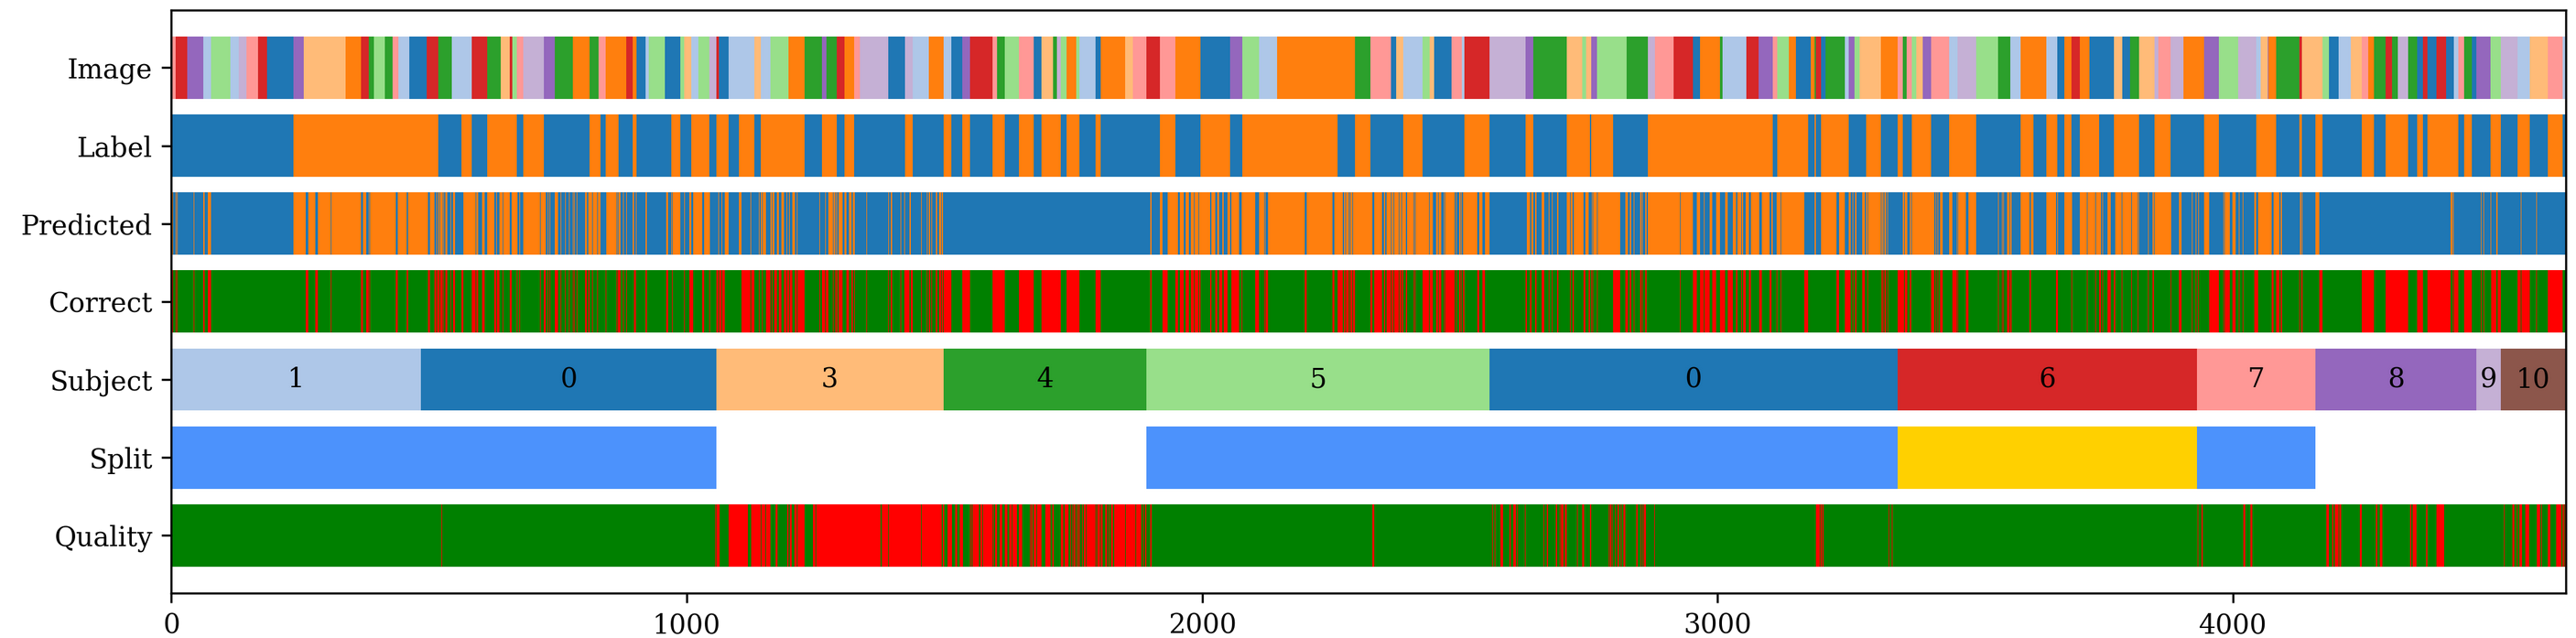
\includegraphics[width=\linewidth]{img/timebars.png}
    \caption{Visualization of the labeled data with classifications from one example subject-fold. Shows the \emph{Image} (stimuli), the class \emph{Label} for that stimuli (\textcolor{NavyBlue}{\textbf{blue}} is code, \textcolor{BurntOrange}{\textbf{orange}} is prose), the \emph{Predicted} class, whether the prediction is \emph{Correct}, the \emph{Subject}, the \emph{Split}/Fold (\textcolor{NavyBlue}{\textbf{blue}} shows the training set, \textcolor{Goldenrod}{\textbf{yellow}} the test set), and our threshold measure for signal \emph{Quality} (\textcolor{Green}{\textbf{green}} indicates acceptable quality). The x-axis is the window index, sorted by acquisition time.
    \\
    \vspace{0.5em}
    It can be seen that (1) subjects \#3 and \#4 have bad signal quality, and have therefore been excluded from the training set. (2) The subjects \#9 and \#10 have also been excluded from training due to issues during data collection. (3) For subject \#1 the stimuli images were not shuffled. (4) Subject \#0 appears twice, as they did two sessions (using unseen stimuli).}\label{fig:timebars}
\end{figure}

        \end{landscape}

        \begin{comment}
            \begin{figure}[h]
            \centering
            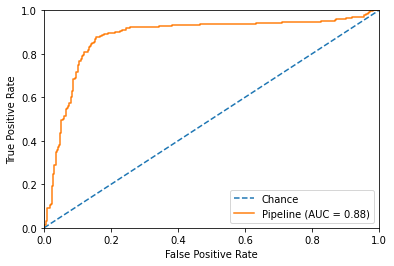
\includegraphics[width=12cm]{img/roccurve.png}
            \caption{Receiver operating characteristic (ROC) curve for subject \#6.}\label{fig:roc}
            \end{figure}
            \change[inline]{Update with higher-res image}
        \end{comment}

    \section{Naturalistic device activity}

        As described in Section~\ref{section:collect-eeg-naturalistic}, we collected approximately \SI{5}{hours} of labeled EEG data using our labels described in Section~\ref{section:collect-usage}. The data was collected on several different days, with a breakdown of the date and class distribution shown in Figure~\ref{figure:dayclass-dist}. 

        Using that data, we trained our classifiers based on Riemannian geometry for each pair of label combinations. The results for each pairing are seen in Table~\ref{table:scores-natural}.

        %\add[inline]{Förklara vad kolumnerna i löptexten så får du lite textvolym. Kan du säga något om när data samlades in? Var det vid ett tillfälle? Flera tillfällen? Tid på dygnet? Eventuellt kan någon sådan metadata även leda till en figur som illustrerar något... Lite deskriptiv statistik kanske finns också? Hur många tillfällen spelades in? Vad var medelvärdet på inspelningstid? Hur såg signalstyrkan ut? Vad triggade dig att sluta spela in? Slut på batteri? Annat? (obekväm sensor, störd av något, eller kände dig färdig)}

        \begin{table}[h]
            \centering
            \begin{tabular}{llrr}
    \toprule
    \textbf{Experiment} & \textbf{Score} & \textbf{Support} & \textbf{Hours} \\
    \midrule
    Programming vs Writing & 0.676 & (1386, 209) & 2.22h \\
    Programming vs Twitter & 0.695 &  (1386, 949) & 3.24h \\
    Programming vs YouTube & 0.672 &  (1386, 266) & 2.29h \\
    Twitter vs Writing & 0.833 &  (949, 209) & 1.61h \\
    Twitter vs YouTube & 0.604 & (949, 266) & 1.69h \\
    YouTube vs Writing & 0.889 &  (266, 209) & 0.66h \\
    \bottomrule
\end{tabular}

            \caption{The scores for each label pairing. The \textit{Score} is the mean balanced accuracy of the StratifiedKFold splits. The \textit{Support} is the number of windows for each class. \textit{Hours} is the sum of both classes' duration.}\label{table:scores-natural}
        \end{table}

        We can see that our balanced accuracy scores are roughly in the same range as the scores achieved in our controlled code vs prose experiment. We note that our naturalistic ``Programming vs Writing'' classifier achieves a \gls{bac} of 0.68, which is slightly worse than the $0.75$ BAC from our controlled experiment. We discuss the results further in \Vref{section:results}.

        \begin{figure}[h]
            \centering
            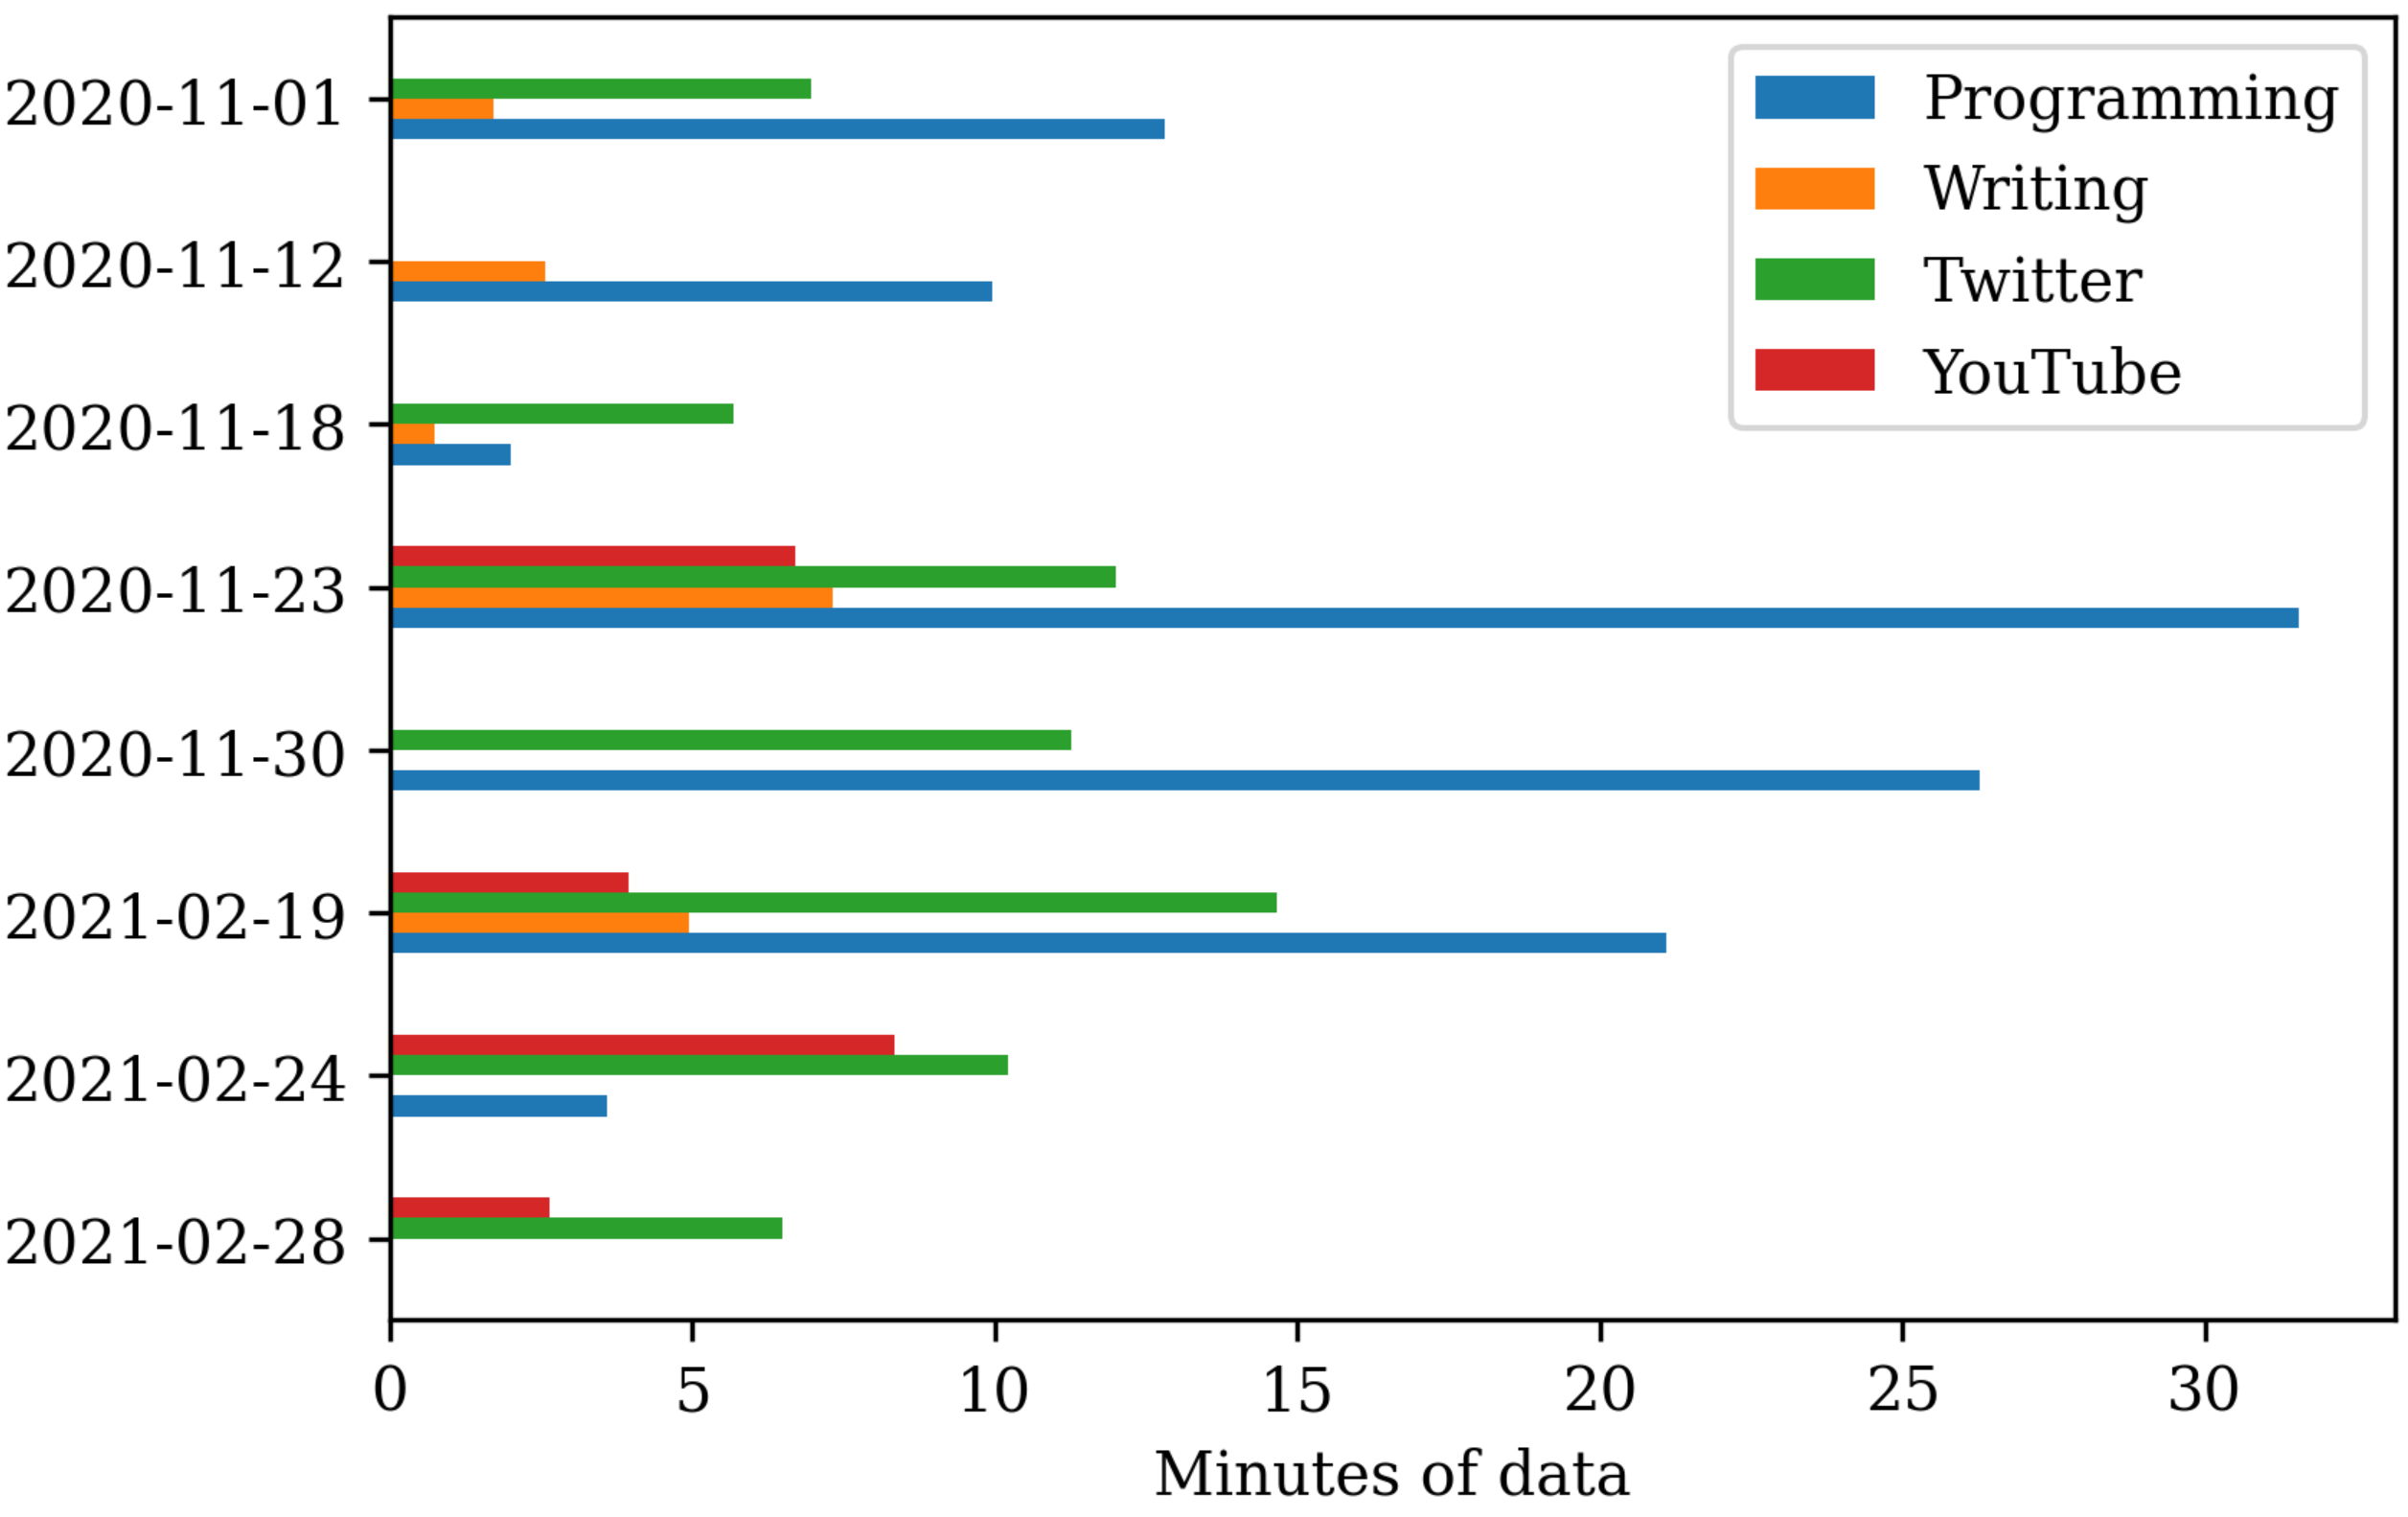
\includegraphics[width=12cm]{img/naturalistic-dayclass-dist.png}
            \caption{Class and date distribution of collected data.}\label{figure:dayclass-dist}
        \end{figure}

        \vfill
